% Pt10a option (a) -- Borrow then Beg. Again only a path of play: B's move
% after Steal is unspecified, so there is no strategy profile to assess.
\documentclass[border=6pt]{standalone}
% ---------------------------------------------------------------------------
% Shared style for ATS1053 extensive-form (game tree) figures.
%
% Companion to matrix-style.tex, and deliberately matching it: sans-serif
% text, mid-grey rules, bold player names. Built compact, so the trees stay
% legible at the ~7cm widths the printed tests use.
%
% Coordinates are plain centimetres. The house layout for a two-stage tree is
%
%     root      (0, 0)
%     depth 1   y = -2.0
%     depth 2   y = -4.0
%
% with siblings 2.6cm apart. Deviate if a figure needs it.
% ---------------------------------------------------------------------------

\usepackage[T1]{fontenc}
\usepackage{helvet}
\renewcommand{\familydefault}{\sfdefault}
\usepackage{tikz}
\usetikzlibrary{arrows.meta,positioning}

\definecolor{gridgrey}{gray}{0.45}
\definecolor{nodefill}{gray}{0.15}

\newcommand{\gtfont}{\fontsize{12}{14}\selectfont}
\newcommand{\gtsmall}{\fontsize{10.5}{12.5}\selectfont}

\tikzset{
  gametree/.style={font=\gtfont, x=1cm, y=1cm},
  % a decision node
  dnode/.style={circle, fill=nodefill, inner sep=0pt, minimum size=3.6mm},
  % the bold player name that sits beside a decision node
  plabel/.style={font=\bfseries\gtfont, inner sep=1.4mm},
  % a branch of the tree
  branch/.style={draw=black, line width=0.85pt,
                 -{Stealth[length=2.2mm,width=1.9mm]}},
  % a branch that has been picked out -- a path of play, or one player's move
  % under some strategy profile
  bbranch/.style={draw=black, line width=2.2pt,
                  -{Stealth[length=3.4mm,width=3.0mm]}},
  % the name of a move, sitting on its branch
  movelabel/.style={font=\gtsmall, inner sep=1mm, fill=white},
  % ditto, on a picked-out branch
  bmovelabel/.style={movelabel, font=\bfseries\gtsmall},
  % a terminal payoff box
  payoff/.style={draw=gridgrey, line width=0.7pt, rectangle, align=center,
                 inner sep=1.7mm, font=\gtsmall, minimum width=9mm},
}

% \pay{a}{b}  -- contents of a payoff box. No player labels: the first mover's
% payoff goes on top, the second mover's underneath, per the house convention.
\newcommand{\pay}[2]{#1\\#2}

% \dn{name}{x}{y}{label}{labelpos}  -- decision node plus its player name
\newcommand{\dn}[5]{%
  \node[dnode] (#1) at (#2,#3) {};%
  \node[plabel, #5=0.5mm of #1] {#4};%
}

% \lf{name}{x}{y}{a}{b}  -- terminal node with payoffs (a, b)
\newcommand{\lf}[5]{\node[payoff] (#1) at (#2,#3) {\pay{#4}{#5}};}

% \mv{from}{to}{label}{labelpos}  -- a branch, labelled with the move
\newcommand{\mv}[4]{%
  \draw[branch] (#1) -- node[movelabel, #4] {#3} (#2);%
}

% \mvb{from}{to}{label}{labelpos}  -- as \mv, but bolded
\newcommand{\mvb}[4]{%
  \draw[bbranch] (#1) -- node[bmovelabel, #4] {#3} (#2);%
}

% \plegend{node}{first}{second}  -- "A:/B:" key to the left of a payoff box,
% for figures where the question text doesn't say whose payoff is whose
\newcommand{\plegend}[3]{%
  \node[font=\gtsmall, align=right, left=1.2mm of #1] {#2:\\#3:};%
}

\begin{document}
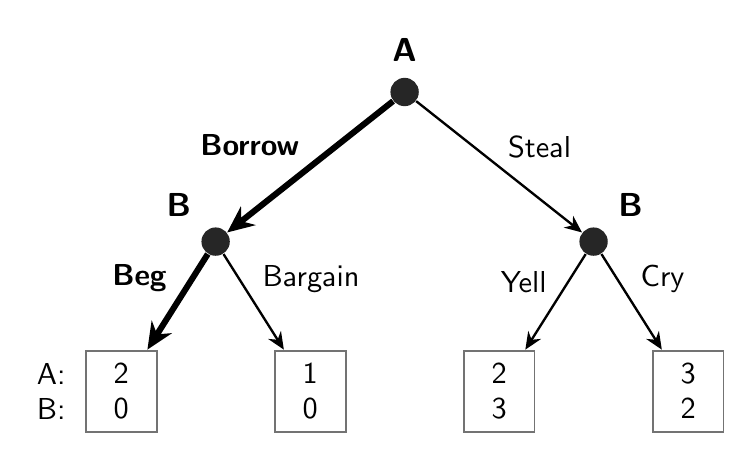
\begin{tikzpicture}[gametree]
  % ---------------------------------------------------------------------------
% Node skeleton for the Borrow/Steal tree -- the one used by Pt10, Pt10a,
% Pt11 and Pt12. Nodes and payoffs only: each figure draws its own branches,
% bolding whichever of them it needs.
%
%                      A
%             Borrow       Steal
%           B                    B
%     Beg     Bargain      Yell     Cry
%    (2,0)     (1,0)      (2,3)    (3,2)
%
% \input this inside a {tikzpicture}[gametree]. Node names: r, bl, br for the
% decision nodes; beg, bar, yel, cry for the leaves.
% ---------------------------------------------------------------------------
  \dn{r}{0}{0}{A}{above}
  \dn{bl}{-2.4}{-1.9}{B}{above left}
  \dn{br}{2.4}{-1.9}{B}{above right}
  \lf{beg}{-3.6}{-3.8}{2}{0}
  \lf{bar}{-1.2}{-3.8}{1}{0}
  \lf{yel}{1.2}{-3.8}{2}{3}
  \lf{cry}{3.6}{-3.8}{3}{2}
  \plegend{beg}{A}{B}

  \mvb{r}{bl}{Borrow}{above left}
  \mv{r}{br}{Steal}{above right}
  \mvb{bl}{beg}{Beg}{above left}
  \mv{bl}{bar}{Bargain}{above right}
  \mv{br}{yel}{Yell}{above left}
  \mv{br}{cry}{Cry}{above right}
\end{tikzpicture}
\end{document}
